% Jellyfish Latency TikZ Figure
% Include directly in main document with \input

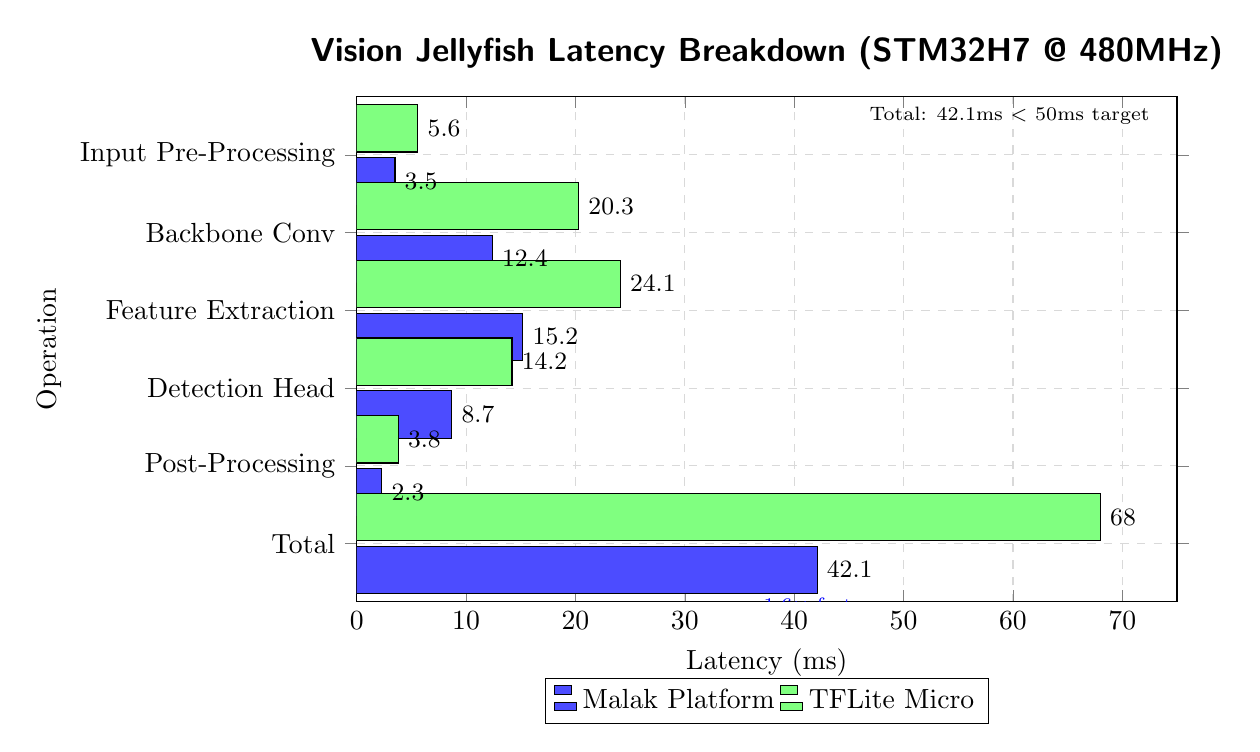
\begin{tikzpicture}
\begin{axis}[
    xbar,
    width=12cm,
    height=8cm,
    xlabel={Latency (ms)},
    ylabel={Operation},
    ytick=data,
    yticklabels={
        Total,
        Post-Processing,
        Detection Head,
        Feature Extraction,
        Backbone Conv,
        Input Pre-Processing
    },
    nodes near coords,
    nodes near coords align={horizontal},
    every node near coord/.append style={font=\small},
    bar width=0.6cm,
    xmin=0,
    xmax=75,
    enlarge y limits=0.15,
    legend style={at={(0.5,-0.15)}, anchor=north, legend columns=2},
    grid=major,
    grid style={dashed, gray!30},
    title={Vision Jellyfish Latency Breakdown (STM32H7 @ 480MHz)},
    title style={font=\large\sffamily\bfseries},
]

\addplot[fill=blue!70, draw=black] coordinates {
    (42.1, 0)
    (2.3, 1)
    (8.7, 2)
    (15.2, 3)
    (12.4, 4)
    (3.5, 5)
};

\addplot[fill=green!50, draw=black] coordinates {
    (68.0, 0)
    (3.8, 1)
    (14.2, 2)
    (24.1, 3)
    (20.3, 4)
    (5.6, 5)
};

\legend{Malak Platform, TFLite Micro}

\node[font=\scriptsize, text=blue] at (axis cs:42.1, -0.8) {1.6$\times$ faster};
\node[font=\scriptsize, anchor=west] at (axis cs:46, 5.5) {Total: 42.1ms $<$ 50ms target \checkmark};

\end{axis}
\end{tikzpicture}
